
%
\documentclass[]{article}
\usepackage{graphicx}  % needed for figures
\usepackage{dcolumn}   % needed for some tables
\usepackage{bm}        % for math
\usepackage{amssymb}   % for math
\usepackage{ifthen}

\usepackage{geometry}
\geometry{legalpaper, portrait, margin=0.75in}

\begin{document}


\title{The LoLIM Impulsive Imager Pipeline}
%\author{P-S.~Laplace}
%\author{S.~Poisson}
%\author{R.~Fisher}
%\author{A.~Kolmogorov}

\date{\today}

%\begin{abstract}
%\end{abstract}

\maketitle

\section{Introduction}

This document explains the use and function of the LoLIM Impulsive Imager Pipeline. Where LoLIM is the LOFAR Lightning Imaging package, which is primarily written in Python, with compute-intensive pieces written in Cython. LOLIM's general use to to assist the LOFAR lightning group to analyze and and plot transient buffer and lightning data from the LOFAR radio telescope. As such it has a wide remit beyond just this one pipeline. All of those additional pieces are not documented here, only the pipeline as that is hard enough. The Impulsive Imager is a very fancy time-of-arrival imager. For every input dataset, the output is a 4D point cloud that shows how that lightning flash develops in space in time. This point cloud is stored as a human-readable text file about 20-100~MB in size. The impulsive imager is briefly described later in this document, but not in great detail. This pipeline is a set of code built around the impulsive imager to automatically run it in an operational mode. That is, to also run all the steps before and after the impulsive imager itself so that impulsively imaged lightning data appears on the LOFAR LTA without very much human intervention. 

I designed this pipeline from scratch myself, as opposed to using a framework, because I do not understand frameworks. I have found that I cannot use something unless I truly and deeply understand the need to do so. In addition, I find using other-peoples code to be an exercise in frustration, as it often takes significant forcing and cludge solutions to make the code work in the way I want and not the way the original designer wanted (if the original designer wanted to do the same things I do then we would not be here). Therefore, I try to not add on such complications unless there is good and obvious reason to do so. Designing and writing this pipeline was relatively straight-forward, thus to this date I still feel no need to use a framework. I should note that this pipeline is relatively straight forward, there are a small number of linearly organized steps, and these steps do not need to be changed thus can be hard-coded into the pipeline. If a more complex or flexible procedure was needed, than I could certainly understand the need for a more professionally written framework. 

\section{Installation}

LoLIM was designed to work with conda, therefore I recommend installing and using conda as the package manager. But this is not necessary. The dependencies for the LoLIM impulsive imager pipeline are:
\begin{itemize}
	\item \textbf{Numpy} Obviously
	\item \textbf{Scipy} 
	\item \textbf{Matplotlib}
	\item \textbf{Pandas} 
	\item \textbf{Cython}
	\item \textbf{h5py} for reading HDF5 format files  
	\item \textbf{GSL}  GNU Scientific Library. A scientific utilities package for C.
\end{itemize}
Note that there is other code in LoLIM that also needs PyQT5. However this is not needed for the pipeline.

After installing dependencies, the first step to installing LoLIM is to unzip the metadata directory ``/path/to/LoLIM/data.tar.xz". So there is a ``data" folder inside LoLIM (note this is a meta-data folder, it is not for experimental data).

Step two is to inform python that LoLIM exists. First way is to use pip. LoLIM comes with a setup.py script that works with pip. Thus one can simply call command:
\begin{verbatim}
pip install /path/to/LoLIM
\end{verbatim}
This install script does very little. Thus, the second way is to install in-place by either placing the path to LoLIM in your bashrc as an environment variable. Or, alternatively, call the python script ``/path/to/LoLIM/install.py" which simply finds where your python installation is and places a symbolic link there.

The third  step of installing LoLIM is building all the cython and C code. There is a built-in python script to do this. Thus this should be as easy as running the following command:
\begin{verbatim}
	python -m LoLIM.build_allCython 
\end{verbatim}




\section{Quick Setup and Operation}

This section will describe how to setup and run the pipeline in the simplest fashion. 

\textbf{Step one: create folders.} Create a folder somewhere it can be held permanently called ``/PATH/lightning". Then create the following sub-folders: ``/PATH/lightning/inject\_LTA\_locations", ``/PATH/lightning/LTA\_locations", ``/PATH/lightning/database" ``/PATH/lightning/raw\_data", and ``/PATH/lightning/processed\_data", where ``PATH'' is the actual path to all of these folders. 

It should be noted that all these folders do not need to be in the same location. It is just easier to explain and start out with. In particular, ``inject\_LTA\_locations" and ``processed\_data'' should be relatively easy to reach, and ``raw\_data" needs to be able to handle large amounts of raw data. 

\textbf{Step two: create settings file.} Find the default settings file at ``/PATH/LoLIM/pipeline/pipelineSettings.JSON". Copy and past this to ``/PATH/lightning/pipelineSettings.JSON". Like folders above, this settings file doesn't literally need to be in the same folder as everything else, but it should be somewhere relatively easily assessable. Next, this pipeline settings file needs to be adjust to meet your needs. The default values of most variables are probably fine. But the following variables in the JSON file need to be set:

\begin{itemize}
	\item \textbf{flashDatabase\_location} set to path of ``database'' folder, followed by ``flashDatabase.json". e.g.: ``/PATH/lightning/database/flashDatabase.json".
	\item \textbf{stormDatabase\_location} ditto but followed by ``stormDatabase.json". e.g.: ``/PATH/lightning/database/stormDatabase.json".
	\item \textbf{raw\_data\_loc} path of raw data folder. e.g.: ``/PATH/lightning/raw\_data".
	\item \textbf{processed\_data\_loc} path of raw data folder. e.g.: ``/PATH/lightning/processed\_data".
	\item \textbf{processor\_uses\_slurm} Set to true if using slurm. If false, pipeline just uses python subprocesses.popen. If a different job manger is desired then the pipeline needs adjusting.
	\item \textbf{slurm\_user} If using SLURM, then this is the user that is calling the pipeline and to add new jobs under.
	\item \textbf{download\_data.LTA\_locations\_folder} the path of the ``LTA\_locations'' folder, e.g.: ``/PATH/lightning/LTA\_locations".
	\item \textbf{download\_data.wgetRC\_file} WGET is used to download data from the LTA. This should be the path of the wgetRC file which should contain a username and password to do so.
\end{itemize}
TODO: add ``inject\_LTA\_locations''. 

\textbf{Step three: Initialize the database.} TODO!!

\textbf{Step four: regularly run the pipeline.} Next, setup the pipeline to be run regularly. E.G. the command:
\begin{verbatim}
	python -m LoLIM.pipeline.processor /PATH/lightning/pipelineSettings.JSON
\end{verbatim}
should be run around once per day. An easy way to do this is to use cron.

\textbf{Step five: inject observations into pipeline.} Observations are injected into the LoLIM Impulsive Imager Pipeline through LTA location files and associated MD5 sum files. It is expected that each observation will produce a single LTA location file with a name that is ``<observation id>.LTAfiles". Where each line in that file is the location of a data file on the LTA. In addition to a HDF5 sum file which has a name ``<observation id>.md5" and each line indicates the MD5 sum of each data file on the LTA. For example, file ``L703974.LTAfiles'' contains the first two lines:
\begin{verbatim}
srm://srm.grid.sara.nl/pnfs/grid.sara.nl/data/lofar/ops/TBB/lightning/L703974_D20190424T194432.504Z_CS001_R000_tbb.h5
srm://srm.grid.sara.nl/pnfs/grid.sara.nl/data/lofar/ops/TBB/lightning/L703974_D20190424T194432.504Z_CS002_R000_tbb.h5
\end{verbatim}
and the file ``L703974.md5'' contains the first two lines:
\begin{verbatim}
98c16c7912c490acd19fe8ba992c64b3  /data/projects/LT10_017/tbb/L703974_D20190424T194432.504Z_CS001_R000_tbb.h5
d3cc4569570184fc8fd36e7ea7e7ab4d  /data/projects/LT10_017/tbb/L703974_D20190424T194432.504Z_CS002_R000_tbb.h5
\end{verbatim}

Observations are injected into the pipeline by simply placing the LTA locations file and md5 sums file into the ``inject\_LTA\_locations'' folder. The next time the processor.py is run it will check this folder, move any files into the ``LTA\_locations'' folder, update the database, and then delete all contents of the  ``inject\_LTA\_locations'' folder. 

After this, all steps of the pipeline ought to run automatically. Including final upload to the LTA. 

\textbf{Step six: inspect pipeline behavior}

TODO! write this section in future once tools are developed.


\section{Pipeline Architecture}

The pipeline has three main pieces: the database, the processor, and the active stages. The database keeps track of which observations (storms) and datasets (flashes) exist, what their names are, and what stage of processing they are in. It should be noted that in the context of this pipeline the word ``storm'' is synonymous with observation and the word ``flash'' is synonymous with dataset (that is, one transient buffer dump including many stations). This is slightly different than the actual geophysical use of those terms, as there can be multiple storms simultaneously (at different places) and there can be multiple lightning flashes in one transient buffer dump. Figure \ref{fig:ThreeComponents} illustrates the relationship between these three components, and the following sections elucidate further.  

\begin{figure}
	\centering
	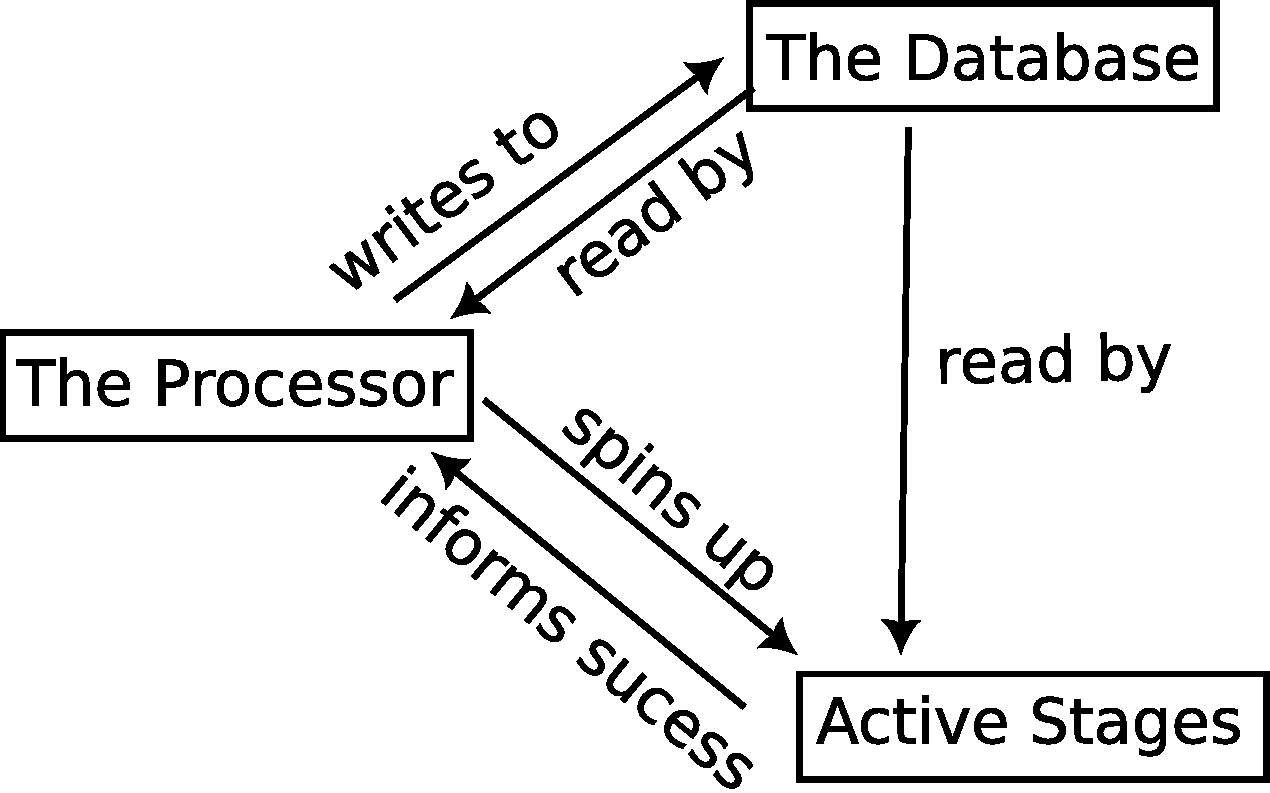
\includegraphics[width=0.7\linewidth]{./figures/TheThreeComponents.pdf}
	\caption{\label{fig:ThreeComponents} The three main components of the pipeline, the database, processor, active stages, and the relationships between the three. }
\end{figure}

\subsection{The Database}

The database keeps track of what storms and flashes exist, what their name is, and what state of processing they are in. In actuality, the database is really two databases; the storm database and the flash database. These are not stored as a SQL database or some other complex nonsense, but as each are simply a Pandas dataframe stored as a JSON. This was chosen for simplicity as something like a SQL database would be significant overkill for this application.

It should be noted that one of the jobs of the database is to track what the name of each storm and flash is. They have a default name of the timeID, which corresponds to the UTC time of their observation. For example,  ``D20190424T194432.504Z" is a lightning flash observed in year 2019, month 4, day 24, hour 19, minute 33, second 32. However, using such a timeID in conversation is a bit awkward, thus each flash also has a name. This flash is named ``19A-1''. The first two digits of this name are obviously the year. The letter indicates the storm where `A' typically means the first storm of the year. However, sometimes in the past storms have been missed entirely and thus this letter can sometimes be out-of-order. The final number, (1), indicates the flash in the storm. In the past assigning such names was done manually, but now this will be done by the database. Obviously, since the name depends on the name of the previous storm and flash, this must be tracked carefully.

\subsubsection{Storm Database}

For the storm database, the index of each row is the storm name, e.g. 19A for the storm that contains the flash 19A-1. The columns of the storm database are:
\begin{itemize}
	\item \textbf{LTAloc\_file} string. Location of the LTA locations file. Note there is a 1-to-1 correlation between a LTA locations file and a storm.
	\item \textbf{MD5Sum\_file} string. Ditto, but for MD5 sums. 
	\item \textbf{year} string. Year of the observation.
	\item \textbf{year} string. Year of the observation.
	\item \textbf{month} string. Month of the observation.
	\item \textbf{day} string. Day of the observation.
	\item \textbf{hour} string. Hour of the observation.
	\item \textbf{ID\_prefix} string. LOFAR observation id. E.g. L2025065
	\item \textbf{numberFlashes} int. Number of flashes in the storm.
\end{itemize}

\subsubsection{Flash Database}

For the flash database the index is the flash name (e.g. 19A-1). The columns are:
\begin{itemize}
	\item \textbf{TimeID} string. e.g. D20190424T194432.504Z
	\item \textbf{year} string
	\item \textbf{month} string
	\item \textbf{day} string
	\item \textbf{state} category, explained further below
	\item \textbf{sub\_state} category, explained further below
	\item \textbf{rawDataDownloaded} bool. Is True if the transient buffer data exists on this server.
	\item \textbf{calibration\_file} string. location and name of the calibration file.
	\item \textbf{pipeline\_priority} int. Priority of this flash in terms of processing. Larger numbers are processed first. default is 5.
	\item \textbf{pipeline\_mode} category, explained more below.
	\item \textbf{deleteData\_on\_complete} bool. Default True. If is true, then when this flash is finished processing (and uploading result to LTA), delete all raw and processed data that is on this server.
	\item \textbf{slurm\_processes} list of integers. Each integer is a CPU or SLURM process ID. Used to check if the process is still running or not. Explained more below. 
	\item \textbf{storm} string. e.g 19A
\end{itemize}

\subsubsection{States and Sub-states}

Every flash has a state, which is essentially just which stage of processing the flash is in. The possible stages are:
\begin{enumerate}
	\item \textbf{ready\_download\_data} Read the LTA locations file and make a small database (in processed files) to track which files are downloaded. In addition to any other small prep work
	\item \textbf{stage\_data} Request data staging on LTA
	\item \textbf{download\_data} Use wget to download data from the LTA
	\item \textbf{initial\_statistics} Perform some initial statistics to find which data blocks have lightning and which do not
	\item \textbf{find\_RFI} Analyze blocks with no lightning to find RFI lines.
	\item \textbf{impulsive\_imager} Run impulsive imager over the data
	\item \textbf{LTA\_upload} Convert native impulsive imager output to a nice text file, upload it to the LTA
	\item \textbf{local\_cleanup} If deleteData\_on\_complete is True, delete all local data.
\end{enumerate}

Every flash also has a sub-state to track the progress of the state the flash is in. There are four sub-states: ready, running, complete, and error. The state transition table is simple. If the flash is in sub-state ready, than the stage is started as a separate set of processes  (CPU threads or SLURM jobs) and the sub-state transitions to running. If the state is running and the processes are all complete, than the sub-state transitions to complete. If the state is complete, the successes of the stage is checked. If the stage was successful then a post-processing function is called. If this function returns True, than the flash state progresses to the next stage and the sub-state transitions to ready. If the stage was not successful or the post-processing function returns False than the sub-state transitions to error. The sub-state error has no transitions.

TODO: include fact that stage can be skipped if it is seen as successfully ran. Include info how this is tracked (e.g. by a file). Probably need to include a figure about the transitions here. 

Every flash has a pipeline\_mode. The typical mode is ``all", where the pipeline runs as normal and all stages are processes. Another mode is ``off'' where the pipeline ignores the flash irregardless of its state (e.g. processing of the flash is complete). All processing stages can also serve as a pipeline\_mode. In such cases the pipeline will perform all stages up to and including the pipeline\_mode stage and then pipeline\_mode is set to ``off''. 



\subsubsection{Accessing and Operating on the Database}

The database is just two text-based JSON files, and thus ostensibly easy to browse and edit with a text editor. This is not recommended. Instead it is strongly recommended to use provided tools. The lowest level tool is a class, LoLIM.pipeline.database.database\_manager. This class is a context manager that attempts to prevent data races with the database between different processes. Example usage is as follows:
\begin{verbatim}
from LoLIM.pipeline import database as DB
with DB.database_manager( PATH_TO_FLASH_DATABASE ) as flash_DB_mangager:
    flash_DB = flash_DB_mangager.read_database()  ## flash_DB is a pandas dataframe
    flash_DB_mangager.save_database( flash_DB )   ## save the DB back to file
\end{verbatim}
The way this context manager works is that it simply checks if a ``lock-file" exists. If the lock file does not exist than the lock file is created and program continues as normal. If the lock file DOES exist, than there is a timeout for a certain time (10 minutes by default), and the lock file is checked again. Once the context manager exits, the lock file is deleted. The lock file is simply an empty file the same name as the provided PATH\_TO\_DATABASE (as in above example) with ``\_lock'' appended to the file name.

A series of command line utilties to inspect the state of the database will be written, and documented here. 

TODO

\subsection{The Processor}

The processor is a python script that reads the database, checks which processes are still running, and decides what state transitions to take. Below is the algorithm that the processor follows.

TODO: I think this algorithm needs a little bit of work...  Need to explain files used to track things are complete. and need to explain job priorities. 

\begin{enumerate}
	\item Backup the database. While the oldest backup is older than settings.maxDatabaseBackup\_Days, delete oldest backup
	\item Search settings.(I forgot name, todo) for new LTA location files, and ingest them into the database.
	\item Read all IDs of all running CPU processes / SLURM jobs.
	\item Loop over every active flash (not mode==``off'',  or sub-state==``error'')
	\begin{enumerate}
		\item If flash sub-state is ``running'', check if any ``slurm\_processes''  are in list of active CPU/SLURM processes. If not, transition sub-state to ``complete''
		
		\item if flash sub-state is ``complete''
		\begin{enumerate}
			\item Check process completed correctly. If not, transition sub-state to ``error''. 
			\item Run post-processing function. If returns False, transition sub-state to ``error''.
			\item Check if there is a following stage in the pipeline.
			\begin{enumerate}
				\item If yes, transition sub-state to ``ready'' and state to the next stage.
				\item If not, set pipeline\_mode to ``off''.
			\end{enumerate}
		
		\end{enumerate}
	
		\item if flash sub-state is ``ready''
		\begin{enumerate}
			\item If stage has already completed successfully, transition sub-state to ``complete''.
			\item Otherwise start up new CPU process/SLURM job to perform the next stage
			\item Add running CPU process IDs / SLURM job IDs to the ``slurm\_processes'' database variable.
		\end{enumerate}
		
	\end{enumerate}
	
\end{enumerate}

Note that the processor will never have more than settings.maxAllowedProcesses running at any one time. 

The processor has two modes to run stages. It can either just spin-up independent processes using python's subprocess.Popen, or it will use SLURM by writing a SLURM job script and call sbatch on it. Note that every stage has a related command that can be run in the terminal. For example, ``python -m LoLIM.pipeline.ready\_download\_data'' is the bash command for the ready\_download\_data stage. After this command, every stage takes five arguments: name of settings JSON file, the flash name, the index of this job, the number of jobs the stage is allowed to use, finally the max allowed number of threads. When the job is complete, it will produce a file with the job number, in the appropriate folder. Thus, the processor just checks that all such files exist to see if the job complete successfully. 

TODO: This needs to be explained a bit more, and also generalized. 

\subsection{The Processing Stages}

TODO be sure to explain the settings. Need somehwere to explain general settings




\end{document}
